\section{Mechanics}
\def\ee{\vc\varepsilon}
\newcommand{\eq}[1]{\begin{equation}#1\end{equation}}
\def\nn{\vc n}
% \def{\tr}{\operatorname{tr}}
\def\uu{\vc u}

Deformation of the porous media is modelled by the stationary linear elasticity equation:
\eq{\label{eq:lin_el} -\div(\delta\tn \sigma(\uu)) = \delta\vc f + \vc f_C + \vc f_H. }
Here $\uu$ \units{}{1}{} is the unknown displacement vector field with 3 components. The stress tensor is given by the Hooke law
\eq{ \tn\sigma(\uu) - \tn\sigma_0 = \tn C\widetilde\ee(\uu) = 2\mu\widetilde\ee(\uu) + \lambda(\tn I:\widetilde\ee(\uu))\tn I }
in terms of the \hyperA{Mechanics-LinearElasticity-FE-Data::initial-stress}{initial stress} $\tn\sigma_0$ [$\mathrm{Pa}$], and the Lam\'e parameters
\eq{ \mu = \frac{E}{2(1+\nu)},\quad \lambda = \frac{E\nu}{(1+\nu)(1-2\nu)}, }
where $E$ [$\mathrm{Pa}$] is the \hyperA{Mechanics-LinearElasticity-FE-Data::young-modulus}{Young modulus} and  $\nu$ \units{}{}{} is the \hyperA{Mechanics-LinearElasticity-FE-Data::poisson-ratio}{Poisson's ratio}.
The strain tensor in $\Omega_d$ is defined as follows:
\eq{ \widetilde\ee(\uu) = \frac12(\nabla\uu_d+\nabla\uu_d^\top) + \begin{cases}0&\mbox{ if }d=3,\\\frac1\delta\sum_{i=1}^n\uu_{d+1}^i\otimes_s\nn_{d+1}^i & \mbox{ else}.\end{cases} }
Here $\vc a\otimes_s\vc b:=\frac12(\vc a\otimes\vc b+\vc b\otimes\vc a)$.

The symbol $\vc f$ stands for the \hyperA{Mechanics-LinearElasticity-FE-Data::load}{body load} [$\mathrm{Nm}^{-3}$].


\paragraph{Hydromechanical coupling.}
The mechanics equation \eqref{eq:lin_el} is coupled to flow by the term
\eq{ \vc f_H = -\nabla(\delta\alpha p), \quad p = \varrho_l g h, }
where $p$ [$\mathrm{Pa}$] is the pressure, $\alpha$ \units{}{}{} is the \hyperA{Coupling-Iterative-Data::biot-alpha}{Biot coefficient}, $\varrho_l$ \units{1}{-3}{} is the \hyperA{Coupling-Iterative-Data::fluid-density}{fluid density} and $g$ \units{}{1}{-2} is the \hyperA{Coupling-Iterative-Data::gravity}{gravitational acceleration}.
Conversely, the deformation affects the flow via the additional term
\eq{\label{eq:fluid_source_div_u} F_M = -\partial_t(\delta\alpha\widetilde\div\uu) }
on the right hand side of \eqref{eq:continuity}.
The expression $\widetilde\div\uu$ is defined as follows:
\eq{ \widetilde\div\uu_d = \div\uu_d + \begin{cases}0 & \mbox{ if }d=3,\\\frac{\delta_{d+1}}{\delta_d}\sum_{i=1}^n\uu^i_{d+1}\cdot\nn^i_{d+1} & \mbox{ else}.\end{cases} }
The numerical solution of coupled hydro-mechanical problems is solved by an iterative splitting, where, in order to achieve convergence, the flow equation is modified as follows:
\eq{ \partial_t(\delta(S+S_{extra})h) + \div\vc q = F + F_M + \partial_t(\delta S_{extra} h_{old}). }
Here $h_{old}$ is the previous value of piezometric head in the iteration process and $S_{extra}$ is an extra storativity coefficient whose value affects the rate of convergence.
It can be manually tuned using the \hyperA{Coupling-Iterative::iteration-parameter}{iteration parameter}.


\paragraph{Boundary conditions.}
Given the decomposition $\partial\Omega_d=\Gamma_D\cup\Gamma_{DN}\cup\Gamma_T\cup\Gamma_S$, we impose the following \hyperA{Mechanics-LinearElasticity-FE-Data::bc-type}{boundary conditions}:
\begin{itemize}
\item \textbf{displacement} condition prescribes
\eq{ \uu = \uu_D \mbox{ on }\Gamma_D }
via \hyperA{Mechanics-LinearElasticity-FE-Data::bc-displacement}{given displacement} $\uu_D$ \units{}{1}{}.
\item \textbf{displacement\_n}: Displacement is prescribed only in the normal component, in tangent directions(s) zero traction is assumed:
\eq{ \left.\begin{aligned}\uu\cdot\nn &= \uu_D\cdot\nn\\
(\sigma(\uu)\nn)_\tau &= \vc 0\end{aligned}\right\} \mbox{ on }\Gamma_{DN}. }
Here $\vc a_\tau := \vc a - (\vc a\cdot\nn)\nn$ is the projection of a vector $\vc a$ to the tangent plane of the boundary.
\item \textbf{traction} condition (default) is imposed via \hyperA{Mechanics-LinearElasticity-FE-Data::bc-traction}{given traction} $\vc t_N$ [$\mathrm{Pa}$]:
\eq{ \sigma(\uu)\nn = \vc t_N \mbox{ on }\Gamma_T. }
\item \textbf{stress} condition is the same type as \textbf{traction}, but instead of traction the user supplies the full \hyperA{Mechanics-LinearElasticity-FE-Data::bc-stress}{stress tensor} $\tn\sigma_N$ [$\mathrm{Pa}$]:
\eq{ \sigma(\uu)\nn = \tn\sigma_N\nn \mbox{ on }\Gamma_S. }
\end{itemize}


\paragraph{Communication between dimensions.}
The mechanical interaction on the interface between $\Omega_{d+1}$ and $\Omega_d$ is realized via the traction condition on the boundary of $\Omega_{d+1}$:
\eq{ \delta_{d+1}(\sigma(\uu^i_{d+1})-\alpha_{d+1}p_{d+1}\tn I)\nn^i_{d+1} = \vc t^i_{d+1,d}, }
where
\eq{ \vc t^i_{d+1,d} = \sigma^U_{d+1,d}\delta_{d+1}\left(\frac{2\delta_{d+1}}{\delta_d}\tn C_d\left((\uu_{d+1}^i-\uu_d)\otimes\nn_{d+1}^i\right)-\alpha_d p_d\tn I\right)\nn_{d+1}^i }
and $\sigma^U_{d+1,d}$ \units{}{}{} is the \hyperA{Mechanics-LinearElasticity-FE-Data::fracture-sigma}{transition coefficient}.
The force term in $\Omega_d$ due to the interaction with $\Omega_{d+1}$ is
\eq{ \vc f_{Cd} = \begin{cases}\vc 0 & \mbox{ if }d=3,\\\sum_{i=1}^n\vc t^i_{d+1,d} & \mbox{ else}.\end{cases} }

\paragraph{Fracture contact mechanics.}
The linear elastic model does not prevent the self-penetration of the deformed porous material.
To avoid this unphysical behaviour, the user has to switch on the \hyperA{Mechanics-LinearElasticity-FE::contact}{contact} parameter.
Then the following contact condition is applied to all fracture elements:
\eq{ \delta_d-\sum_{i=1}^n\delta_{d+1}^i\uu_{d+1}^i\cdot\nn_{d+1}^i \ge \delta_{contact}, }
where $\delta_{contact}$ is the minimal cross-section of the fracture.
In the case $d=2$, the minimal cross-section is just the contact distance.
For $1d$ fractures/channels $\delta_{min}$ corresponds to the minimal contact area.

The real fracture surface is never flat. To simulate the roughness of the fracture, we use the following shear dilation model.
If the rock surfaces adjacent to the fracture move in tangential direction, then the minimal contact distance increases according to the formula:
\eq{ \delta_{contact} = \delta_{min} + \min\{\tan(\alpha_{rough}) j_\tau,\delta_{rough}\}, }
where $\delta_{min}$ \units{}{3-d}{} is the \hyperA{Mechanics-LinearElasticity-FE-Data::cross-section-min}{minimal cross-section},
$\alpha_{rough}$ \units{}{}{} is the \hyperA{Mechanics-LinearElasticity-FE-Data::roughness-angle}{roughness angle} (in radians),
$\delta_{rough}$ \units{}{3-d}{} is the \hyperA{Mechanics-LinearElasticity-FE-Data::roughness-height}{roughness height}
and $j_\tau$ \units{}{3-d}{} is the jump of tangential displacements of adjacent rock blocks (see Figure \ref{fig:shear_dilation} for illustration).
\begin{figure}
\centering
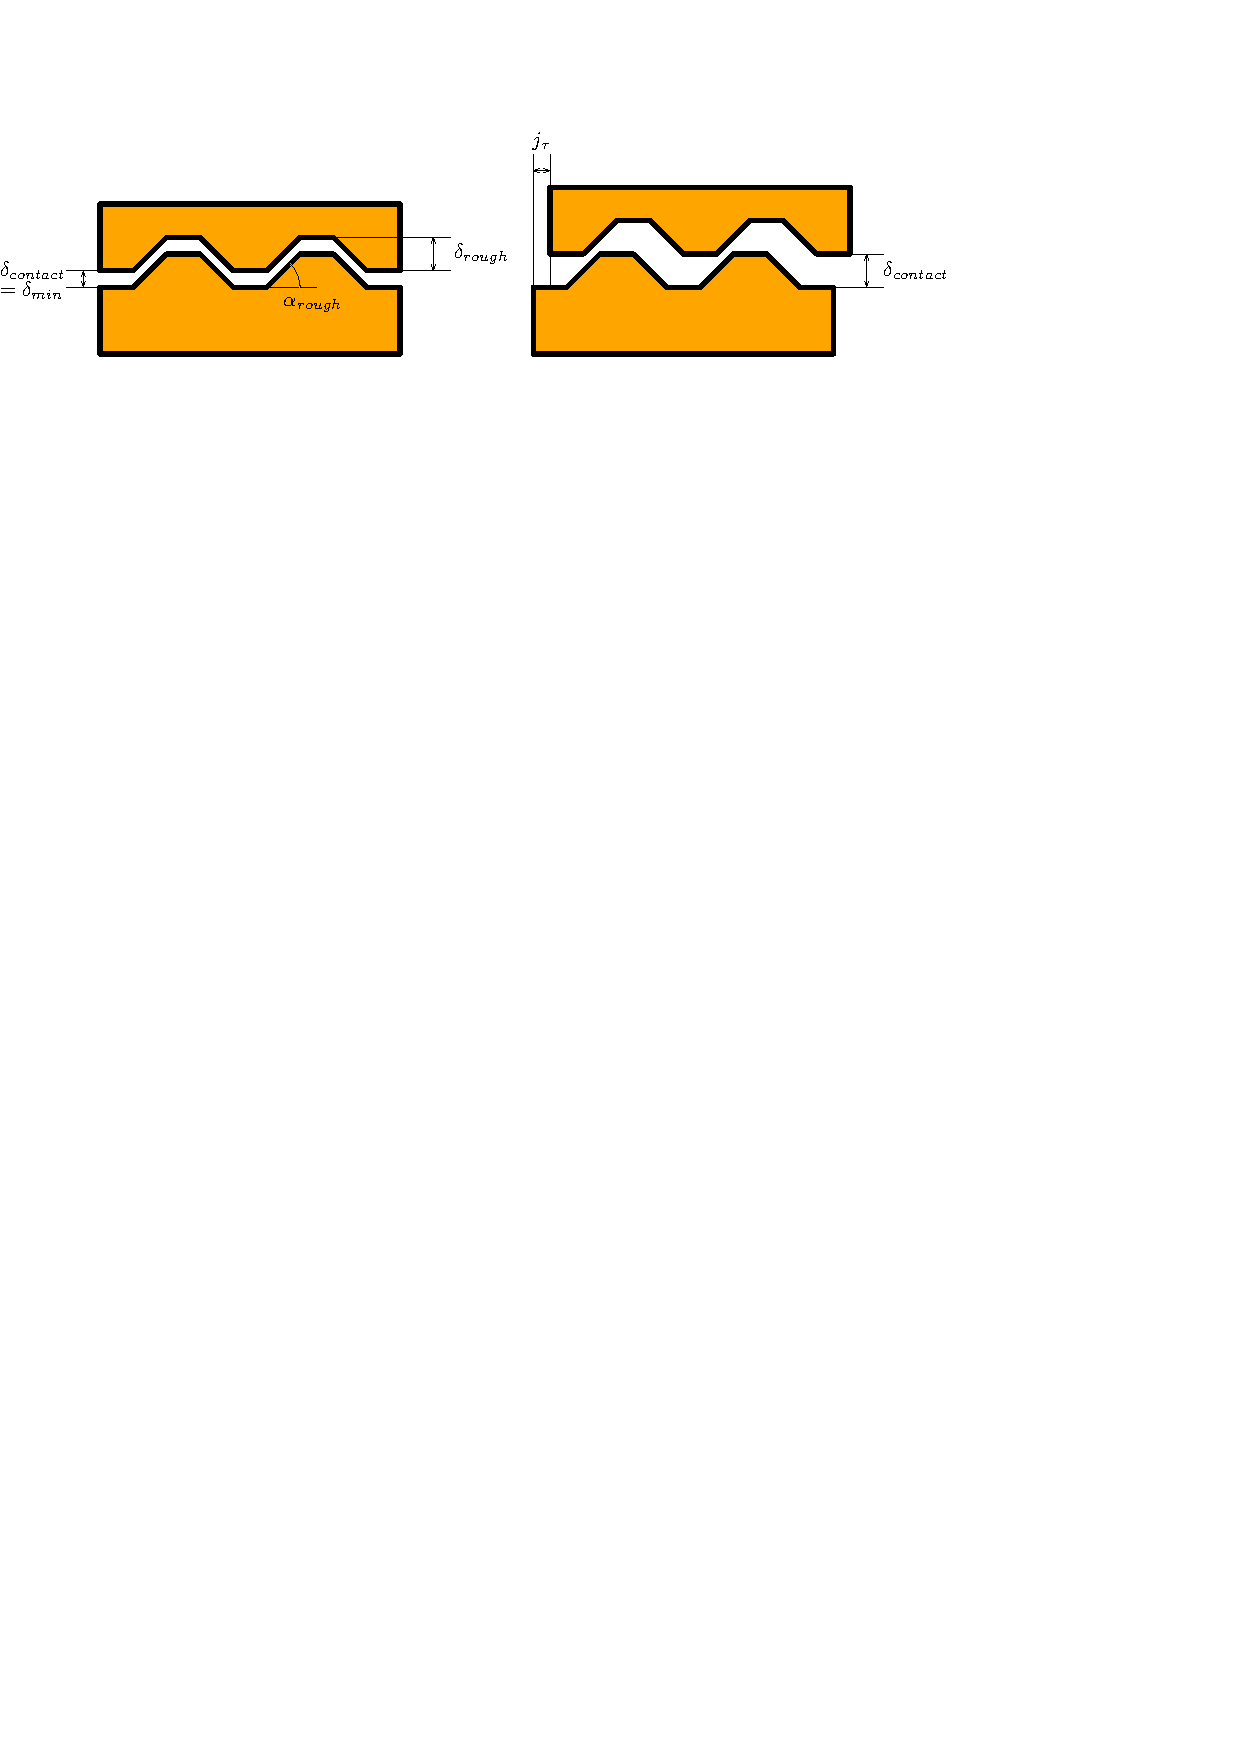
\includegraphics{figures/shear_dilation}
\caption{Ilustration of shear dilation effect: The contact distance increases with tangential displacement.}
\label{fig:shear_dilation}
\end{figure}
For the case of 1d intersections of three or more 2d fractures, $j_\tau$ is generalized to the following formula:
\eq{ j_\tau = \sqrt{ \sum_{i,j=1}^n \delta^i\delta^j(\uu^i_{\tau}\cdot\uu^j_{\tau}) (\nn^i\cdot\nn^j), } }
where $\uu_{i\tau}$ is the tangential displacement on $i$-th branch.

When contact conditions are active, the mechanical model is solved as a quadratic programming problem with linear constraints.

\paragraph{Output fields.}
The mechanics equation provides several fields for output:
\begin{itemize}
    \item \hyperA{Mechanics-LinearElasticity-FE-OutputFields::displacement}{displacement}: The computed displacement vector field $\uu$;
    \item \hyperA{Mechanics-LinearElasticity-FE-OutputFields::stress}{stress}: The mechanical stress tensor $\tn\sigma(\uu)$;
    \item \hyperA{Mechanics-LinearElasticity-FE-OutputFields::mean-stress}{mean\_stress}: The mean of the principal stresses, i.e. $\sigma_m:=\frac13\tn I:\tn\sigma(\uu)$;
    \item \hyperA{Mechanics-LinearElasticity-FE-OutputFields::von-mises-stress}{von\_mises\_stress}: $\sigma_{VM}:=\sqrt{\frac32\tn\sigma_d:\tn\sigma_d}$, where $\tn\sigma_d:=\tn\sigma(\uu)-\sigma_m\tn I$ is the deviatoric stress.
    Equivalently, von Mises stress can be expressed as
    \[ \sigma_{VM} = \sqrt{\frac12\left((\sigma_1-\sigma_2)^2+(\sigma_1-\sigma_3)^2+(\sigma_2-\sigma_3)^2\right)}, \]
    where $\sigma_{1,2,3}$ are the principal stresses, i.e. eigenvalues of $\tn\sigma(\uu)$;
    \item \hyperA{Mechanics-LinearElasticity-FE-OutputFields::cross-section-updated}{cross\_section\_updated}: This field expresses the cross-section of fractures after deformation and is defined as $\delta_d-\sum_{i=1}^n\uu^i_{d+1}\cdot\nn^i_{d+1}$;
    \item \hyperA{Mechanics-LinearElasticity-FE-OutputFields::displacement-divergence}{displacement\_divergence}: $\widetilde\div\uu_d$;
    \item \hyperA{Mechanics-LinearElasticity-FE-OutputFields::normal-displacement-jump}{normal\_displacement\_jump}: Displacement jump in normal direction: $\sum_{i=1}^n\uu^i_{d+1}\cdot\nn^i_{d+1}$;
    \item \hyperA{Mechanics-LinearElasticity-FE-OutputFields::tangential-displacement-jump}{tangential\_displacement\_jump}: Displacement jump in tangential direction ($j_\tau$).
\end{itemize}

